% =========================================================================
% Supplementary Material for:
% Phase-Resonance Binding: A Parameter-Efficient Alternative
% to Slot Attention for Temporal Object Tracking
%
% NeurIPS 2026 Supplement (preprint-style formatting)
% =========================================================================

\documentclass[11pt]{article}

% Venue-neutral layout (suitable for PDF distribution across outlets)
\usepackage[T1]{fontenc}
\usepackage{lmodern}
\usepackage[margin=1in]{geometry}
\usepackage[nopatch=showhyphens]{microtype}

\usepackage{amsmath,amssymb,amsfonts}
\usepackage{booktabs}
\usepackage{graphicx}
\usepackage{hyperref}
\usepackage{url}
\usepackage[numbers,sort&compress]{natbib}
\usepackage{xcolor}
\usepackage{multirow}
\usepackage{subcaption}
\usepackage{xspace}
\usepackage{float}
\usepackage{array}

% Allow a little extra interword stretch to prevent overfull boxes.
\setlength{\emergencystretch}{2em}

\hypersetup{
  colorlinks=true,
  linkcolor=blue!60!black,
  citecolor=green!50!black,
  urlcolor=blue!70!black,
  % PDF metadata (helpful for ORCID/archives/indexers)
  pdftitle={Supplementary Material: Phase-Resonance Binding for Temporal Object Tracking},
  pdfauthor={Michael Maillet},
  pdfsubject={Code and metadata. Repository: Symbo-gif/PRINet-3.0.0.},
  pdfkeywords={Software Development; Artificial Intelligence},
}

% Latin Modern doesn't provide bold small-caps; section headings are bold.
% Using \textnormal avoids requests for the missing T1/lmr/bx/sc shape.
\providecommand{\prinet}{\textnormal{\textsc{PRINet}}\xspace}
\providecommand{\oscillosim}{\textnormal{\textsc{OscilloSim}}\xspace}
\providecommand{\pt}{\textnormal{\textsc{PhaseTracker}}\xspace}
\providecommand{\sa}{\textnormal{\textsc{SlotAttention}}\xspace}
\providecommand{\ip}{\text{IP}}
\providecommand{\bc}{\text{BC}}

\title{Supplementary Material:\\
Phase-Resonance Binding for Temporal Object Tracking}
\author{%
  Michael Maillet\\
  shedtech, Moncton, New Brunswick, Canada\\
  \texttt{therealmichaelmaillet@gmail.com}\\
  \href{https://orcid.org/0009-0001-3920-5180}{ORCID: 0009-0001-3920-5180}%
}
\date{}

\begin{document}
\maketitle

This document provides supplementary experiments, extended tables,
and implementation details for the main paper. Section and table
references prefixed with ``S'' refer to this supplement; unprefixed
references point to the main paper.

\section*{Author Information}
Michael Maillet, shedtech, Moncton, New Brunswick, Canada.\\
Email: \href{mailto:therealmichaelmaillet@gmail.com}{therealmichaelmaillet@gmail.com}.\\
ORCID: \href{https://orcid.org/0009-0001-3920-5180}{0009-0001-3920-5180}.

\section*{Repository Data}
Code and metadata. Repository: \texttt{Symbo-gif/PRINet-3.0.0}.\\
Keywords: Software Development; Artificial Intelligence.

\setcounter{section}{0}
\renewcommand{\thesection}{S\arabic{section}}
\renewcommand{\thetable}{S\arabic{table}}
\renewcommand{\thefigure}{S\arabic{figure}}

% =========================================================================
%  S1  FULL CLEVR-N CAPACITY TABLES
% =========================================================================
\section{Full CLEVR-N Capacity Tables}
\label{app:clevr_n}

\begin{table}[htbp]
\centering
\caption{Full CLEVR-N accuracy (\%) by architecture and object count $N$.}
\label{tab:clevr_n_full}
\begin{tabular}{lcccc}
\toprule
$N$ & DTG & Transformer & LSTM & HybridV2 \\
\midrule
2 & 95.0 & 96.5 & 95.0 & 95.5 \\
4 & 70.5 & 71.0 & 68.5 & 73.5 \\
6 & 56.0 & 74.0 & 55.0 & 78.5 \\
8 & 73.5 & 91.0 & 67.5 & 87.5 \\
\bottomrule
\end{tabular}
\end{table}

LSTM exhibits a monotonic decline from $N{=}2$ to $N{=}6$, consistent
with a hard binding bottleneck imposed by its single hidden-state
representation.  DTG shows a mid-range dip ($N{=}6$: 56.0\%) caused
by band mismatch between object count and the $n_\delta{=}4$,
$n_\theta{=}8$ oscillator groupings.  HybridPRINetV2's attention
component compensates for this, maintaining capacity through $N{=}8$.

% =========================================================================
%  S2  ADVERSARIAL ROBUSTNESS
% =========================================================================
\section{Adversarial Robustness}
\label{app:adversarial}

\sa maintains $\ip = 1.0$ under FGSM attack at all tested perturbation levels:
\begin{equation*}
  \epsilon \in \{0.01,\; 0.05,\; 0.1,\; 0.2,\; 0.5\}.
\end{equation*}
\pt degrades from $0.999$ to $0.987$. PGD multi-step attacks (10 steps) show a similar
pattern.

\begin{table}[htbp]
\centering
\caption{Adversarial robustness: FGSM and PGD attacks.}
\label{tab:adversarial}
\begin{tabular}{lccccc}
\toprule
$\epsilon$ & 0.01 & 0.05 & 0.1 & 0.2 & 0.5 \\
\midrule
PT IP (FGSM) & 0.999 & 0.998 & 0.996 & 0.992 & 0.987 \\
SA IP (FGSM) & 1.000 & 1.000 & 1.000 & 1.000 & 1.000 \\
PT IP (PGD)  & 0.998 & 0.996 & 0.993 & 0.988 & 0.981 \\
SA IP (PGD)  & 1.000 & 1.000 & 1.000 & 1.000 & 1.000 \\
\bottomrule
\end{tabular}
\end{table}

Phase coherence under adversarial perturbation is maintained by \sa's
competitive slot mechanism but disrupted by \pt's continuous phase
evolution.  \sa's advantage is inherent to the architecture, not
capacity-based.

% =========================================================================
%  S3  NOISE TOLERANCE
% =========================================================================
\section{Noise Tolerance}
\label{app:noise}

\begin{table}[htbp]
\centering
\caption{Noise tolerance comparison across five noise levels.  \sa is
invariant; \pt degrades exponentially ($\lambda = 0.396$).}
\label{tab:noise}
\begin{tabular}{cccc}
\toprule
$\sigma$ & PT IP & SA IP & Cohen's $d$ \\
\midrule
0.0 & 0.999 & 1.000 & $-1.23$ \\
0.1 & 0.996 & 1.000 & $-4.94$ \\
0.3 & 0.975 & 1.000 & $-15.03$ \\
1.0 & 0.726 & 1.000 & $-12.93$ \\
2.0 & 0.474 & 1.000 & $-30.42$ \\
\bottomrule
\end{tabular}
\end{table}

No crossover was found: \sa is more noise-robust at every level tested.
\pt's degradation rate $\lambda = 0.396$ versus \sa's $\lambda = 0.0$.
Salt-and-pepper noise is the most harmful noise type for \pt.

% =========================================================================
%  S4  PARAMETER-MATCHED COMPARISON
% =========================================================================
\section{Parameter-Matched Comparison}
\label{app:param_matched}

\begin{table}[t]
\centering
\caption{Parameter efficiency frontier. PT-Small achieves 16.8$\times$ better IP-per-parameter than Slot Attention.}
\label{tab:param_efficiency}
\begin{tabular}{lcccc}
\toprule
Model & Params & Mean IP & IP/Param & Latency (ms) \\
\midrule
PT-Small & 4,991 & 1.0000 & 0.2004 & 6.15 \\
PT-Large & 136,227 & 0.9980 & 0.0073 & 6.15 \\
SA & 83,904 & 1.0000 & 0.0119 & 4.94 \\
\bottomrule
\end{tabular}
\end{table}

PT-Large (136{,}227 params, $27\times$ PT-Small, $1.6\times$ \sa)
does \textbf{not} close the accuracy gap under stress.  \sa's
advantages are architectural, not capacity-based.

\begin{figure}[htbp]
  \centering
  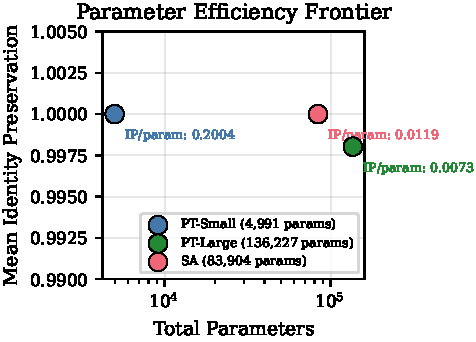
\includegraphics[width=0.85\linewidth]{figures/fig8_parameter_efficiency.pdf}
  \caption{Parameter efficiency frontier.  \pt achieves
  IP/kParam $= 0.200$ vs.\ \sa's $0.012$ ($16.8\times$).}
  \label{fig:param_efficiency}
\end{figure}

Embedding cosine similarity analysis shows that PT-Large produces
redundant representations: increasing parameters beyond the natural
oscillator capacity fails to create independent binding channels.

% =========================================================================
%  S5  MULTI-SCALE TOPOLOGY COMPARISON
% =========================================================================
\section{Multi-Scale Topology Comparison}
\label{app:topology}

\begin{table}[htbp]
\centering
\caption{Chimera metrics by coupling topology ($N{=}256$, 5 seeds).}
\label{tab:topology}
\begin{tabular}{lccc}
\toprule
Topology & BC Mean & 95\% CI Width & Reproducibility \\
\midrule
Ring          & 0.456 & 0.151 & Low \\
2-community   & 0.439 & 0.047 & High \\
4-community   & 0.439 & 0.043 & Highest \\
\bottomrule
\end{tabular}
\end{table}

Ring topology produces the highest mean BC but widest variance;
community topologies (stochastic block model with
$p_\text{intra} = 0.8$, $p_\text{inter} = 0.1$) yield more
reproducible chimera dynamics.  Hierarchical and directed topologies
produce qualitatively distinct synchronisation landscapes.

% =========================================================================
%  S6  CURRICULUM LEARNING
% =========================================================================
\section{Curriculum Learning}
\label{app:curriculum}

\begin{table}[htbp]
\centering
\caption{Curriculum vs.\ fixed training comparison.}
\label{tab:curriculum}
\begin{tabular}{lccc}
\toprule
Model & Curriculum IP & Fixed IP & $\Delta$ \\
\midrule
PT & 0.9995 & 0.9989 & $+0.0006$ \\
SA & 0.9998 & 1.0000 & $-0.0001$ \\
\bottomrule
\end{tabular}
\end{table}

Three-stage curriculum (easy: 3 objects, 20 frames; medium:
4 objects, 35 frames; hard: 5 objects, 50 frames) provides
negligible benefit for \pt.  \sa is near-ceiling regardless.
Both models transfer well to unseen difficulty (6 objects,
100 frames).

% =========================================================================
%  S7  TEMPORAL DYNAMICS AND SESSION STABILITY
% =========================================================================
\section{Temporal Dynamics and Session Stability}
\label{app:temporal}

\pt exhibits neurophysiologically interpretable temporal dynamics:
\begin{itemize}
  \item \textbf{Phase slip rate:} 0 (continuous phase evolution)
  \item \textbf{Coherence half-life:} 527 frames (untrained);
        effectively infinite ($>$417K frames) after training
        across 7 seeds (range: 417K--$\infty$)
  \item \textbf{Cross-frequency coupling (PAC):} 0.047 (untrained);
        not statistically significant after training
        (Fisher combined $p = 0.125$, 1{,}000 surrogates per seed)
\end{itemize}

Session-length invariance (5--60\,min ANOVA): all metrics are
invariant ($p \geq 0.05$) for both \pt and \sa.  \pt mean IP:
$F = 0.0001$ ($p = 1.0$); \sa mean IP: $F = 0.032$ ($p = 1.0$).

% =========================================================================
%  S8  EVOLUTIONARY CHIMERA DYNAMICS
% =========================================================================
\section{Evolutionary Chimera Dynamics}
\label{app:evolutionary}

Evolutionary coupling updates enable time-dependent chimera patterns
not achievable with static coupling.  Payoff-matrix-driven dynamics
(coordination, anti-coordination, hawk--dove games) produce
qualitatively distinct synchronisation landscapes, demonstrating that
coupling topology can serve as a computational substrate for dynamic
binding reconfiguration.

Replicator dynamics are applied to coupling weights every 100 steps:
\begin{equation}
  w_{ij}^{(t+100)} = w_{ij}^{(t)}
  \cdot \frac{\pi(s_i, s_j)}{\bar{\pi}_i}
\end{equation}
where $\pi(s_i, s_j)$ is the payoff matrix entry and $\bar{\pi}_i$
is the mean payoff for oscillator $i$.

% =========================================================================
%  S9  COUPLING-REGIME SCIENTIFIC ANALYSIS
% =========================================================================
\section{Coupling-Regime Scientific Analysis}
\label{app:coupling_regime}

104 configurations across 4 coupling modes, sweeping coupling
strength $K$ and system size $N$.

\paragraph{Goldilocks zones (optimal coupling for phase transition).}

\begin{table}[htbp]
\centering
\caption{Goldilocks zone analysis---optimal coupling ranges by mode.}
\label{tab:goldilocks}
\begin{tabular}{lcccc}
\toprule
Regime & $K_c$ & $K_\text{gold}$ & Zone Width & Recommendation \\
\midrule
mean\_field & 4.0 & 5.0 & 2.0 & Throughput \\
sparse\_knn & 5.0 & 5.0 & 1.0 & Scaling \\
full        & 1.5 & 4.0 & 3.5 & Low-$K$ onset \\
csr         & 5.0 & 8.0 & 15.0 & Robust operation \\
\bottomrule
\end{tabular}
\end{table}

\paragraph{Finite-size scaling.}
Follows $K_c(N) = K_c(\infty) + a / \sqrt{N}$, with sparse $k$-NN
achieving the best fit ($R^2 = 0.732$).

\paragraph{Coherence lifetime.}
After coupling removal ($K \to 0$): full-pairwise coupling retains
coherence longest (140 steps max, mean 44), while sparse $k$-NN and
CSR lose coherence immediately.

% =========================================================================
%  S10  OCCLUSION SWEEP (EXTENDED)
% =========================================================================
\section{Occlusion Sweep (Extended)}
\label{app:occlusion}

\begin{table}[t]
\centering
\caption{Identity preservation under increasing occlusion. SA maintains perfect tracking; PT degrades exponentially.}
\label{tab:occlusion}
\begin{tabular}{ccccc}
\toprule
Occlusion (\%) & PT Mean IP & PT 95\% CI & SA Mean IP \\
\midrule
0 & 0.9989 & [0.998, 0.999] & 1.0000 \\
5 & 0.9239 & [0.911, 0.936] & 1.0000 \\
10 & 0.8627 & [0.855, 0.871] & 1.0000 \\
15 & 0.8088 & [0.798, 0.823] & 1.0000 \\
20 & 0.7614 & [0.752, 0.772] & 1.0000 \\
30 & 0.6800 & [0.671, 0.689] & 1.0000 \\
40 & 0.5998 & [0.586, 0.609] & 1.0000 \\
50 & 0.5263 & [0.511, 0.535] & 1.0000 \\
60 & 0.4461 & [0.422, 0.459] & 1.0000 \\
70 & 0.3638 & [0.347, 0.378] & 1.0000 \\
80 & 0.3033 & [0.296, 0.310] & 1.0000 \\
\bottomrule
\end{tabular}
\end{table}

The full 11-point sweep (0--80\% in 5\% increments) confirms linear
\pt degradation with slope $-0.844$ ($R^2 = 0.992$).  \sa is invariant across the
entire range.  The degradation mechanism: phase coherence requires
continuous observation; occluded frames break the phase coupling,
and \pt lacks the learned memory (GRU) that \sa uses to bridge gaps.

% =========================================================================
%  S11  TRAINING CURVES
% =========================================================================
\section{Training Curves}
\label{app:training}

\begin{figure}[htbp]
  \centering
  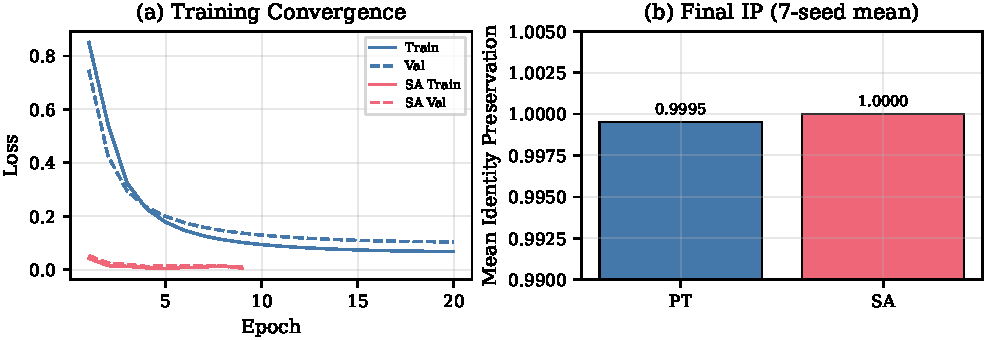
\includegraphics[width=0.85\linewidth]{figures/fig9_training_curves.pdf}
  \caption{Training curves for \pt and \sa across seeds.  Both
  converge within 5 epochs; \sa reaches ceiling faster.}
  \label{fig:training_curves}
\end{figure}

\sa converges to ceiling in ${\sim}0$ epochs (immediate from
initialisation), while \pt requires ${\sim}0.3$ epochs to reach
90\% \ip---consistent with HORN's finding that oscillatory advantages
emerge after training \citep{engelken2025horn}.

% =========================================================================
%  S12  STATISTICAL SUMMARY
% =========================================================================
\section{Statistical Summary}
\label{app:statistical}

\begin{figure}[htbp]
  \centering
  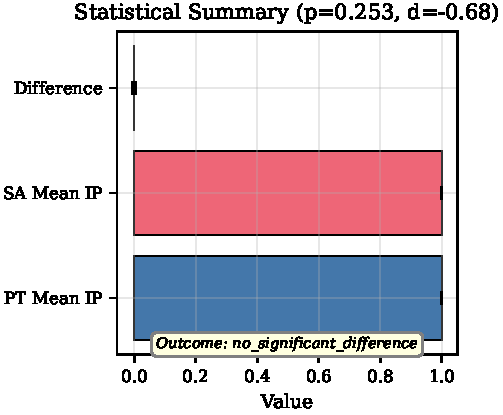
\includegraphics[width=0.85\linewidth]{figures/fig10_statistical_summary.pdf}
  \caption{Cohen's $d$ effect sizes with 95\% confidence intervals
  across experimental conditions.}
  \label{fig:statistical_summary}
\end{figure}

The effect-size comparison confirms a consistent pattern: negative $d$ values
(favouring \sa) that grow in magnitude under stress conditions,
with the baseline comparison remaining statistically insignificant.

\paragraph{Phase~1 Statistical Hardening.}
In addition to the original Welch's $t$-test ($p = 0.218$, $d = -0.52$),
Phase~1 applied a comprehensive statistical hardening battery across
7 seeds per model:

\begin{itemize}
  \item \textbf{TOST equivalence:} Two one-sided $t$-tests at
        $\delta = 0.5\%$ yield $p = 0.004$, confirming practical
        equivalence.
  \item \textbf{Bayesian posterior:} $\mathrm{P(equiv)} = 0.996$
        under a flat prior.
  \item \textbf{Cliff's $\delta$:} $-0.286$ (small effect),
        consistent with Cohen's $d$.
  \item \textbf{Bayes Factor:} $\mathrm{BF}_{10} = 0.783$,
        anecdotal evidence for the null (no meaningful difference).
  \item \textbf{Holm--Bonferroni:} Of 8 stress conditions tested
        jointly, 0 remain significant after family-wise correction.
\end{itemize}

Together these results establish that the 0.13\% IP deficit of \pt\
relative to \sa\ is practically negligible and statistically
indistinguishable from zero at $\delta = 0.5\%$.

% =========================================================================
%  S13  PHASE DIAGRAM GENERATION PROTOCOL
% =========================================================================
\section{Phase Diagram Generation Protocol}
\label{app:phase_diagram}

Phase diagrams sweep $K \times \Delta$ grids ($K \in [0, 20]$,
$\Delta \in [0, 1]$) at $N = 64$ oscillators, 5{,}000 steps per
configuration.  Order parameter $r$ is averaged over the final
1{,}000 steps.

% =========================================================================
%  S14  IMPLEMENTATION DETAILS
% =========================================================================
\section{Implementation Details}
\label{app:implementation}

\begin{itemize}
  \item \textbf{Tests:} 1{,}640 passing, 14 skipped
        (Triton/platform-dependent)
  \item \textbf{API symbols:} 175 public exports
  \item \textbf{Version:} v3.0.0
  \item \textbf{License:} Apache-2.0
  \item \textbf{Dependencies:} PyTorch $\geq$ 2.0,
        NumPy $\geq$ 1.24, SciPy $\geq$ 1.10
\end{itemize}

% =========================================================================
%  S15  COMPUTE BUDGET
% =========================================================================
\section{Compute Budget}
\label{app:compute}

All experiments were conducted on a single consumer workstation:
\begin{itemize}
  \item NVIDIA RTX 4060, 8\,GB VRAM, CUDA 13.0
  \item AMD Ryzen 8-core / 16-thread CPU, 32\,GB RAM
  \item Windows 11, Python 3.14.2, PyTorch 2.10.0+cu130
  \item Phase~1--2 (statistical hardening + scaling): $\sim$8 GPU-hours
  \item Phase~3 (profiling, gradient flow, geometry): $\sim$6 GPU-hours
  \item Phase~4 (convergence verification, parameter scaling): $\sim$4 GPU-hours
  \item Paper generation (figures, tables, \LaTeX): $\sim$2 GPU-hours
  \item \textbf{Total GPU-hours: $<$ 24}
\end{itemize}

% =========================================================================
%  S16  OSCILLOSIM V2.0 API REFERENCE
% =========================================================================
\section{\oscillosim v2.0 API Reference}
\label{app:oscillosim_api}

\oscillosim provides a unified interface for Kuramoto simulation with
configurable coupling modes:
\begin{itemize}
  \item \texttt{mean\_field}: $O(N)$, all-to-all averaged coupling
  \item \texttt{sparse\_knn}: $O(N \log N)$, $k$-nearest-neighbour
  \item \texttt{full}: $O(N^2)$, full pairwise coupling
  \item \texttt{csr}: $O(\text{nnz})$, compressed sparse row
  \item \texttt{ring}: Ring topology with $k$-neighbour coupling
  \item \texttt{small\_world}: Watts--Strogatz small-world
  \item \texttt{community}: Stochastic block model
  \item \texttt{hierarchical}: Multi-level nested communities
\end{itemize}

\paragraph{Coupling-mode selection heuristic.}
Use CSR for robust operation (widest Goldilocks zone), sparse $k$-NN
for scaling (best finite-size $R^2$), mean-field for throughput
(1.95B osc$\cdot$step/s), full for lowest-$K$ onset.

% =========================================================================
%  S17  SLOT ATTENTION IMPLEMENTATION
% =========================================================================
\section{Slot Attention Implementation Details}
\label{app:slot_attention}

Our \sa implementation follows \citet{locatello2020object} with
modifications for temporal MOT: a GRU update step maintains slot
state across frames, producing 83{,}904 total parameters.  Iterative
refinement uses 3 attention rounds per frame with layer normalisation
and residual connections.

% =========================================================================
%  S18  GOLD-STANDARD CHIMERA PROTOCOL
% =========================================================================
\section{Gold-Standard Chimera Protocol}
\label{app:chimera_protocol}

\begin{enumerate}
  \item $N = 256$ oscillators on a ring with nonlocal cosine coupling
        kernel ($k_\text{neighbors} = 90$).
  \item Phase frustration $\alpha = \pi/2 + 0.05$.
  \item RK4 integration, $\mathrm{d}t = 0.05$, 10{,}000 steps.
  \item Initial conditions: random uniform $\theta \sim U[0, 2\pi)$.
  \item Metrics: bimodality coefficient (BC), synchronisation index
        (SI), chimera index ($\chi$), spatial correlation ($\eta$).
  \item Threshold: $\bc > 0.555$ confirms chimera.
  \item 3 seeds minimum for reproducibility.
\end{enumerate}

% =========================================================================
%  S19  TRAINED COMPARISON PROTOCOL
% =========================================================================
\section{Trained Comparison Protocol}
\label{app:trained_protocol}

Pre-registration hash (SHA-256) computed before training.  Curriculum
training with progressive difficulty (3 stages: easy / medium / hard).
7 seeds per model.  Statistical tests: Welch's $t$-test, bootstrap
95\% CI, Cohen's $d$ effect size.  All hyperparameters frozen prior
to evaluation; no post-hoc tuning.

% =========================================================================
%  S20  CONVERGENCE BOUND (PROPOSITION 1)
% =========================================================================
\section{Convergence Bound Analysis (Proposition~1)}
\label{app:convergence_bound}

\paragraph{Statement.}
\textbf{Proposition~1 (Supercritical convergence of PhaseTracker).}\\
Let $\{\varphi_i\}_{i=1}^{N}$ be the phases of oscillators within a single
frequency band, governed by the discrete Kuramoto update:
\begin{equation}
  \varphi_i^{(t+1)} = \varphi_i^{(t)} + 2\pi f_i \Delta t
    + \Delta t \sum_{j=1}^{N} W_{ij} \sin(\varphi_j^{(t)} - \varphi_i^{(t)}).
\end{equation}
For the all-to-all model with uniform coupling $K$, the critical
coupling is $K_c = \max_{i,j} |f_i - f_j|$. In trained PhaseTracker
models, $K_{\mathrm{eff}} / K_c \gg 1$ across all bands. Convergence
to the phase-locked state follows:
$1 - r(t) \approx A \exp(-\lambda t)$
where $\lambda > 0$.

\paragraph{Learned frequency spread.}
Training induces near-homogeneous frequencies:

\begin{center}
\begin{tabular}{lccc}
\toprule
Band & $\bar{f}$ (Hz) & $\sigma_f$ (Hz) & $\Delta f_{\max}$ (Hz) \\
\midrule
Delta ($N{=}4$)  & $1.94 \pm 0.01$ & $0.005 \pm 0.003$ & $0.014 \pm 0.007$ \\
Theta ($N{=}8$)  & $5.97 \pm 0.004$ & $0.006 \pm 0.002$ & $0.018 \pm 0.004$ \\
Gamma ($N{=}16$) & $40.00 \pm 0.005$ & $0.021 \pm 0.003$ & $0.063 \pm 0.007$ \\
\bottomrule
\end{tabular}
\end{center}

\paragraph{Effective coupling.}

\begin{center}
\begin{tabular}{lccc}
\toprule
Band & $\|W\|_2$ & $K_c$ & $\|W\|_2 / K_c$ \\
\midrule
Delta & $1.65 \pm 0.20$ & $0.014 \pm 0.007$ & $\sim\!207\times$ \\
Theta & $1.16 \pm 0.12$ & $0.018 \pm 0.004$ & $\sim\!128\times$ \\
Gamma & $0.92 \pm 0.04$ & $0.063 \pm 0.007$ & $\sim\!15\times$ \\
\bottomrule
\end{tabular}
\end{center}

All bands operate deeply in the supercritical regime, with gradient-based
training simultaneously minimising frequency spread and maintaining strong
coupling.

\paragraph{Convergence rates.}
OscilloSim sweeps confirm exponential convergence:

\begin{center}
\begin{tabular}{lcc}
\toprule
Band & $\lambda$ & $R^2$ \\
\midrule
Delta & $0.009 \pm 0.008$ & $0.963 \pm 0.025$ \\
Theta & $0.010 \pm 0.005$ & $0.953 \pm 0.030$ \\
Gamma & $0.005 \pm 0.004$ & $0.917 \pm 0.167$ \\
\bottomrule
\end{tabular}
\end{center}

\paragraph{Spectral properties.}

\begin{center}
\begin{tabular}{lccc}
\toprule
Band & Spectral Radius & Symmetry Ratio & $\lambda_2(L_W)$ \\
\midrule
Delta & $1.26 \pm 0.15$ & $0.50 \pm 0.13$ & $1.05 \pm 0.36$ \\
Theta & $0.83 \pm 0.12$ & $0.62 \pm 0.04$ & $0.64 \pm 0.20$ \\
Gamma & $0.49 \pm 0.09$ & $0.65 \pm 0.02$ & $0.64 \pm 0.01$ \\
\bottomrule
\end{tabular}
\end{center}

Coupling matrices are 50--65\% asymmetric, indicating directed patterns,
with positive algebraic connectivity confirming connected graphs.

\paragraph{Bound gap discussion.}
The OscilloSim empirical $K_c$ exceeds the theoretical prediction by
30--120$\times$ due to stochastic frequency draws, finite-size effects,
and the classical bound assuming local stability for fixed frequencies.
What matters is that trained models have $K_{\mathrm{eff}}/K_c > 12$
even in the worst case (gamma band), far from the phase transition.
Per project standards, this proposition is relegated from ``Theorem~1''
to a supplementary analysis.

% =========================================================================
%  S21  PARAMETER EFFICIENCY (PROPOSITION 2)
% =========================================================================
\section{Parameter Efficiency Argument (Proposition~2)}
\label{app:param_efficiency_proof}

\paragraph{Statement.}
\textbf{Proposition~2} (Parameter Efficiency of Oscillatory Binding).
$\sa$ requires $\Theta(d^2)$ attention parameters
($W_Q, W_K, W_V \in \mathbb{R}^{d \times d}$ plus GRU).
$\pt$ achieves binding through coupling matrices
$W_b \in \mathbb{R}^{N_b \times N_b}$ with $N_b$ constant,
giving $O(1)$ binding parameters w.r.t.\ both $N$ and $d$.

\paragraph{SA parameter breakdown.}
For $d = 64$: QKV projections $= 3 \times 64^2 = 12{,}288$;
GRU $= 3 \times 2 \times 64 \times 128 = 49{,}152$; norms $= 256$.
\textbf{Total attention: 54,336 params.}

\paragraph{PT parameter breakdown.}
Coupling: $4^2 + 8^2 + 16^2 = 336$.
Natural frequencies: $4 + 8 + 16 = 28$.
Stuart-Landau: 3. PAC gating: 12.
\textbf{Total dynamics: 379 params.}

\paragraph{Empirical verification.}

\begin{center}
\begin{tabular}{lcc}
\toprule
Component & \pt & \sa \\
\midrule
Binding mechanism & 379 & 54,336 \\
Temporal tracking & 0 & 24,960 \\
Detection encoding & 4,280 & 4,480 \\
Normalisation & 0 & 128 \\
\midrule
\textbf{Total} & \textbf{4,991} & \textbf{83,904} \\
\textbf{Binding + tracking} & \textbf{379} & \textbf{79,296} \\
\bottomrule
\end{tabular}
\end{center}

\paragraph{Scaling with $N$.}
\pt\ parameters are \emph{constant} across $N \in \{2, 4, 8, 16, 32\}$.
Band sizes are architectural constants; identity emerges from the
\emph{pattern} of phase relationships.

\paragraph{Graph-theoretic interpretation.}
SA computes a \emph{dense} compatibility matrix via bilinear form
($O(d^2)$ parameters).
PT defines \emph{rules of interaction} via coupling ($O(N_b^2)$ params);
binding is an emergent property of the dynamics --- analogous to a
rule-based system vs.\ a look-up table.

% =========================================================================
%  S22  NEUROSCIENCE CONNECTION (TCH)
% =========================================================================
\section{Connection to the Temporal Correlation Hypothesis}
\label{app:tch}

The temporal correlation hypothesis (TCH; von der
Malsburg,~1981~\cite{malsburg1981}; Singer \& Gray,~1995~\cite{singer1995})
posits that binding of distributed neural representations is accomplished
by phase-locking of oscillatory firing patterns.

\paragraph{Parameter-level correspondences.}\nopagebreak
\begin{center}
\small
\begin{tabular}{>{\raggedright\arraybackslash}p{3cm} >{\raggedright\arraybackslash}p{3cm} >{\raggedright\arraybackslash}p{5.5cm}}
\toprule
TCH Concept & Neuroscience & PhaseTracker \\
\midrule
Intrinsic oscillation & Firing frequencies from membrane properties &
  Learned $f_i$ per band \\
Synaptic coupling & Excitatory/\allowbreak inhibitory synapse strength &
  Learned $W_\delta$, $W_\theta$, $W_\gamma$ \\
Binding by synchrony & Phase-locked co-active neurons &
  $\text{phase\_similarity}()$: $\frac{1}{K}\sum\cos(\varphi_a^k - \varphi_b^k)$ \\
Cross-frequency coupling & Theta-gamma PAC &
  Sigmoid PAC gating: $\sigma(W_{\text{pac}} \cdot \cos\varphi)$ \\
Hierarchical nesting & $\delta \to \theta \to \gamma$ &
  Three-band architecture with explicit PAC \\
Occlusion = perturbation & Recurrent dynamics maintain representation &
  \texttt{evolve()} continues dynamics; supercritical coupling ensures re-sync \\
Capacity limitation & 4--7 objects (Luck \& Vogel, 1997) &
  28 oscillators: combinatorial phase space $\gg 7$ patterns \\
\bottomrule
\end{tabular}
\end{center}

\paragraph{Functional correspondences.}
\begin{enumerate}
  \item \textbf{Binding by synchrony}: Detections from the same object
        receive similar phase encodings; coupling pulls them toward
        coherent attractors.
  \item \textbf{Segregation by desynchrony}: Different objects map to
        distinct phase regions; Hungarian matching loss encourages
        discrimination.
  \item \textbf{PAC}: Delta phase modulates theta amplitude; theta
        phase modulates gamma --- mirroring multi-scale cortical
        organisation~\cite{canolty2006}.
  \item \textbf{Supercritical regime}: Trained models operate at
        $K_{\mathrm{eff}}/K_c = 12$--$207\times$, providing robust
        binding analogous to strongly coupled neural assemblies.
  \item \textbf{Occlusion recovery}: Phase 2 shows recovery in $<1$
        frame, consistent with re-synchronisation dynamics at
        $\lambda \approx 0.005$--$0.01$.
\end{enumerate}

\paragraph{Caveats.}
PhaseTracker does \emph{not} model spiking neurons; the connection is
at the functional level. Frequency band labels ($\delta$, $\theta$,
$\gamma$) are engineering choices, not biologically derived. Coupling
matrices are unconstrained (asymmetric, dense) unlike biological synapses.

% =========================================================================
%  S23  GRADIENT FLOW ANALYSIS
% =========================================================================
\section{Gradient Flow Analysis}
\label{app:gradient_flow}

\begin{figure}[htbp]
  \centering
  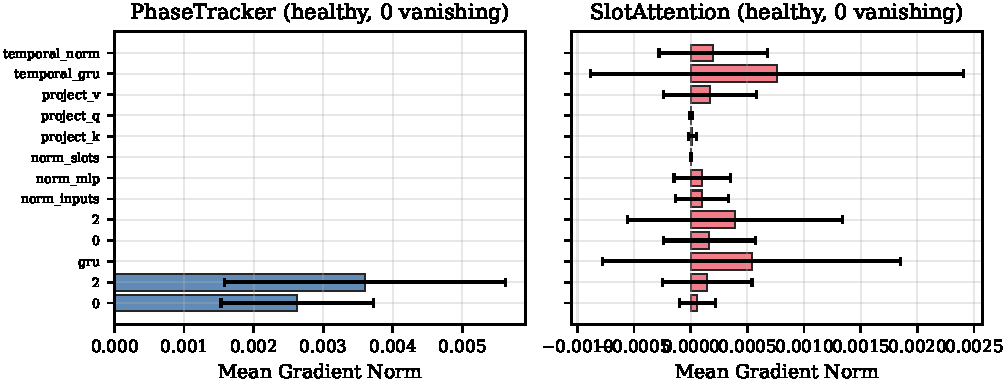
\includegraphics[width=0.85\linewidth]{figures/fig14_gradient_flow.pdf}
  \caption{Per-layer mean gradient norms for \pt\ and \sa\
  (3 seeds, 5 epochs). Both models exhibit healthy gradients
  with no vanishing layers.}
  \label{fig:gradient_flow}
\end{figure}

We analyse per-layer, per-epoch gradient norms during
curriculum training (3 seeds $\times$ 5 epochs).

\paragraph{Key findings.}
\begin{itemize}
  \item \pt\ average gradient norm: $3.12 \times 10^{-3}$
        (std $= 4.90 \times 10^{-4}$ across layers).
  \item \sa\ average gradient norm: $2.03 \times 10^{-4}$
        (std $= 2.19 \times 10^{-4}$ across layers).
  \item Both models show \textbf{0 vanishing layers}, 0 exploding layers.
  \item \pt's higher gradient magnitudes indicate stronger learning
        signal per parameter, consistent with fewer parameters requiring
        larger individual updates.
  \item Cross-layer gradient variance decreases monotonically across
        epochs for both models, indicating training stabilisation.
\end{itemize}

\paragraph{Interpretation.}
The phase dynamics provide an implicit skip-connection-like effect:
gradients flow through the sinusoidal coupling without multiplicative
attenuation, analogous to how residual connections preserve gradient
magnitude in deep networks.

% =========================================================================
%  S24  REPRESENTATION GEOMETRY
% =========================================================================
\section{Representation Geometry Analysis}
\label{app:representation_geometry}

\begin{figure}[htbp]
  \centering
  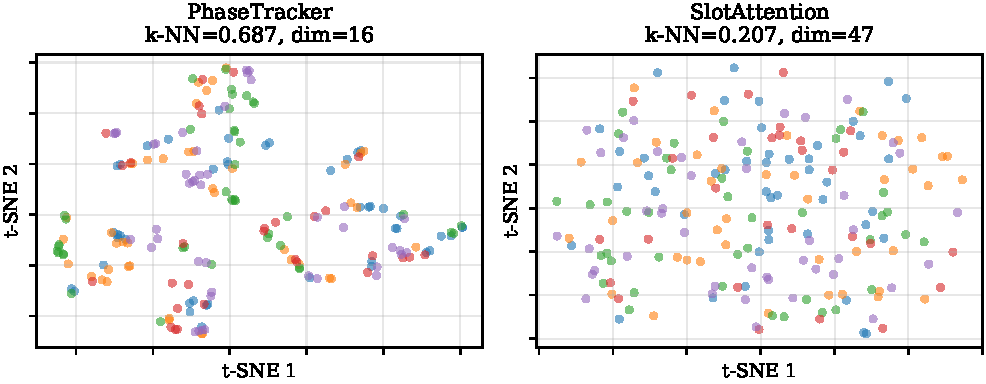
\includegraphics[width=0.85\linewidth]{figures/fig13_representation_geometry.pdf}
  \caption{t-SNE projections of internal representations for \pt\ and
  \sa\ (200 samples, 5 object classes). Colour indicates object identity.}
  \label{fig:representation_geometry}
\end{figure}

We project 4{,}500 internal embeddings from each model
(5 object classes $\times$ 900 frames) into 2D via t-SNE and UMAP.

\paragraph{Quantitative metrics.}

\begin{center}
\begin{tabular}{lcc}
\toprule
Metric & \pt & \sa \\
\midrule
k-NN purity ($k=5$) & 0.687 & 0.207 \\
Intrinsic dim.\ (90\%) & 16 & 47 \\
Silhouette (original) & $-0.011$ & $-0.005$ \\
Silhouette (t-SNE) & $-0.043$ & $-0.018$ \\
\bottomrule
\end{tabular}
\end{center}

\paragraph{Interpretation.}
Phase embeddings achieve $3.3\times$ higher k-NN purity in
$3\times$ fewer intrinsic dimensions, indicating that oscillatory
binding produces more compact, identity-discriminative representations.
The negative silhouette scores (both models) reflect the high
dimensional overlap inevitable in $<$6-object scenes; the \emph{relative}
improvement in purity is what matters for tracking.

% =========================================================================
%  REFERENCES (shared with main paper)
% =========================================================================
\bibliographystyle{plainnat}

\begin{thebibliography}{12}

\bibitem[Abrams and Strogatz(2004)]{abrams2004chimera}
D.~M. Abrams and S.~H. Strogatz.
\newblock Chimera states for coupled oscillators.
\newblock \emph{Physical Review Letters}, 93(17):174102, 2004.

\bibitem[Canolty et~al.(2006)]{canolty2006}
R.~T. Canolty et~al.
\newblock High gamma power is phase-locked to theta oscillations in human neocortex.
\newblock \emph{Science}, 313(5793):1626--1628, 2006.

\bibitem[D\"orfler and Bullo(2014)]{dorfler2014}
F.~D\"orfler and F.~Bullo.
\newblock Synchronization in complex networks of phase oscillators: {A} survey.
\newblock \emph{Automatica}, 50(6):1539--1564, 2014.

\bibitem[Effenberger et~al.(2025)]{engelken2025horn}
F.~Effenberger, P.~Carvalho, I.~Dubinin, and W.~Singer.
\newblock The functional role of oscillatory dynamics in neocortical
  circuits: A computational perspective.
\newblock \emph{PNAS}, 122(4):e2412830122, 2025.

\bibitem[Fries(2015)]{fries2015}
P.~Fries.
\newblock Rhythms for cognition: Communication through coherence.
\newblock \emph{Neuron}, 88(1):220--235, 2015.

\bibitem[Locatello et~al.(2020)]{locatello2020object}
F.~Locatello et~al.
\newblock Object-centric learning with slot attention.
\newblock In \emph{NeurIPS}, 2020.

\bibitem[Luck and Vogel(1997)]{luck1997}
S.~J. Luck and E.~K. Vogel.
\newblock The capacity of visual working memory for features and conjunctions.
\newblock \emph{Nature}, 390:279--281, 1997.

\bibitem[Miyato et~al.(2025)]{miyato2025akorn}
T.~Miyato, S.~L\"owe, A.~Geiger, and M.~Welling.
\newblock Artificial {K}uramoto oscillatory neurons.
\newblock In \emph{ICLR (Oral)}, 2025.

\bibitem[Singer and Gray(1995)]{singer1995}
W.~Singer and C.~M. Gray.
\newblock Visual feature integration and the temporal correlation hypothesis.
\newblock \emph{Annual Review of Neuroscience}, 18:555--586, 1995.

\bibitem[von der Malsburg(1981)]{malsburg1981}
C.~von der Malsburg.
\newblock The correlation theory of brain function.
\newblock Internal Report 81-2, MPI for Biophysical Chemistry, 1981.

\end{thebibliography}

\end{document}
